\section{Statistical Analysis}
\label{sec:analysis}

In this section, we delve into a comprehensive analysis of the retrieval effectiveness for our 5 different runs submitted to \ac{CLEF} on both the French and English collections (see Table \ref{tab:run_parameters}). 
The analysis aims to evaluate the performance of different runs and provides insights into the effectiveness of the system in retrieving and ranking relevant documents.

We begin by analyzing the results obtained from the French collection. 
The overall \ac{nDCG} and \ac{MAP} comparison allows us to gain an initial understanding of the performance differences between runs 2, 3, and 5, considering short-term, heldout, and long-term evaluations. 
By examining the \ac{nDCG} scores and \ac{RnD} values, we can identify the run that demonstrates the highest effectiveness in retrieving relevant documents.

Furthermore, we employ two-way \ac{ANOVA} tests to investigate the significance of the observed differences in the long-term and short-term evaluations. 
This analysis provides valuable insights into the performance of the \ac{IR} system on the French collection, guiding us in identifying areas for improvement.

Subsequently, we shift our focus to the analysis of results obtained from the English collection. 
We conduct an analogous evaluation, comparing the performance of runs 1 and 4 in the same way as stated above for the French collection. 

The analyses and discussions provided in the next subsections aim to give a better understanding of the performance of the developed \ac{IR} system and serve as a basis for optimizing its retrieval performances.


\newpage
\subsection{Analysis of Results on the French Collection}
\enlargethispage{5\baselineskip}
\subsubsection{Overall \textit{nDCG} Comparison}  \label{sec:ndcg_comparison_french}

The overall \ac{nDCG} comparison of Runs 2, 3, and 5 on the French collection is presented in Figure \ref{fig:overall_ndcg_french_boxplot}. 
This boxplot provides valuable insights into the performance of each run, with the bars representing the \ac{nDCG} scores for each run. 
The color coding distinguishes the different evaluation periods, with short-term depicted in green, heldout in orange, and long-term in pink. 
The delta values within the boxes represent the \ac{RnD} of each run compared to the heldout run.

\begin{figure}[!h]
\centering
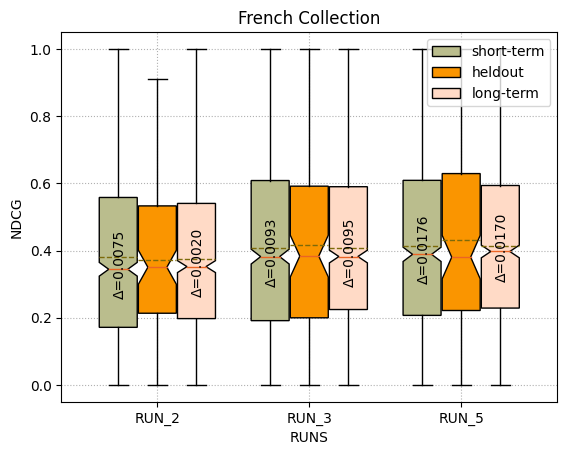
\includegraphics[width=0.8\textwidth]{figure/StatisticalAnalysis/BoxPlot/NDGC French.png}
\caption{Overall \ac{nDCG} Comparison for Runs 2, 3, and 5 on the French Collection}
\label{fig:overall_ndcg_french_boxplot}
\end{figure}

Analyzing the overall \ac{nDCG} comparison, we observe that Runs 3 and 5 consistently outperform Run 2 across both short and long-term evaluations. 
These runs achieve higher \ac{nDCG} scores, indicating their superior effectiveness in capturing relevant documents. 
The fact that both Runs 3 and 5 exhibit similar levels of performance suggests comparable retrieval capabilities among these two.

However, when considering the \ac{RnD} values, we observe some variations among the runs. 
Run 5 demonstrates a noticeable drop in \ac{nDCG} compared to the heldout run, as indicated by the \ac{RnD} delta values. 
This indicates a potential decrease in retrieval performance when transitioning from the heldout period to the short and long term.

On the other hand, Run 3 displays a relatively smaller drop in \ac{nDCG} compared to the heldout run, suggesting greater stability and consistency in capturing relevant documents over time.

In contrast, Run 2 exhibits relatively lower \ac{nDCG} scores, particularly in the long-term evaluation. This can be attributed to its more greedy approach, which might compromise its ability to retrieve relevant documents as the collection evolves over time.


\newpage
\enlargethispage{5\baselineskip}
\subsubsection{Overall \textit{MAP} Comparison}
The boxplot shown in Figure \ref{fig:map_french} presents the overall \ac{MAP} comparison of Runs 2, 3, and 5 on the French Collection.
The notation for the used colors is the same as for Figure \ref{fig:overall_ndcg_french_boxplot}.
From the boxplot, we can observe the distribution of \ac{MAP} scores for each run and collection type. The height of each box indicates the \ac{IQR}, representing the range of the middle 50\% of the data. 
The horizontal line within each box corresponds to the median value, while the whiskers above and below the box extend to the highest and lowest values within 1.5 times the \ac{IQR}.

\begin{figure}[!h]
    \centering
    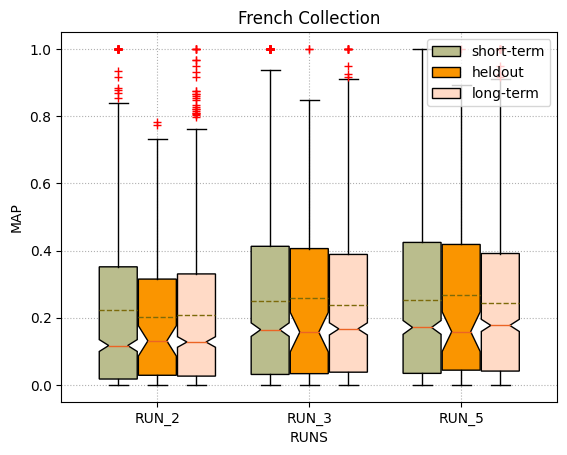
\includegraphics[width=0.8\textwidth]{figure/StatisticalAnalysis/BoxPlot/MAP French.png}
    \caption{Overall MAP Comparison of Runs 2, 3, and 5 on the French Collection}
    \label{fig:map_french}
\end{figure}

Analyzing the overall \ac{nDCG} comparison, we observe that Runs 3 and 5 consistently outperform Run 2 across both short and long-term evaluations, similarly to what we have seen in Section \ref{sec:ndcg_comparison_french}.
These runs achieve higher \ac{nDCG} scores, indicating their superior effectiveness in capturing relevant documents.  

However, we can see that Run 5 demonstrates a noticeable drop in \ac{nDCG} of the long-term compared to the heldout run. 
This indicates a potential decrease in retrieval performance when transitioning from the heldout period to the long term. 
On the other hand, Run 3 displays a relatively smaller drop in \ac{nDCG} compared to the heldout run, suggesting greater stability and consistency in capturing relevant documents over time.

In contrast, Run 2 exhibits relatively lower \ac{nDCG} scores, particularly in the long-term evaluation. This can be attributed to its more greedy approach, which might compromise its ability to retrieve relevant documents as the collection evolves over time.

Overall, these results confirm what we found in Section \ref{sec:ndcg_comparison_french}: Runs 3 and 5 are competitive with each other, while Run 2 exhibits lower performances compared to these, due to its more basic implementation (see Table \ref{tab:run_parameters}). 


\subsubsection{Two-way \textit{ANOVA} on the Long Term French Collection} \label{sec:anova_fr_lt}

The results of the two-way \ac{ANOVA} conducted on the Long Term French Collection are depicted in Figure \ref{fig:lt_anova_french}, which showcases the mean \ac{nDCG} and \ac{AP} scores for Run 2 in red, Run 3 in grey, and Run 5 in blue. 
This plot enables us to examine the effects of both the run choice and the long-term evaluation on the performances.

\begin{figure}[!h]
    \centering
    \begin{subfigure}[b]{0.49\textwidth}
      \centering
      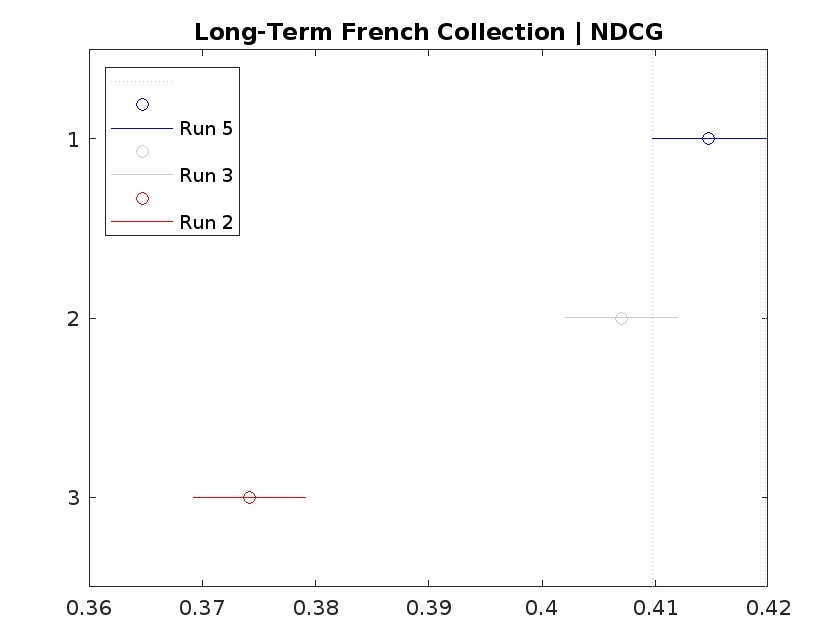
\includegraphics[width=\textwidth]{figure/StatisticalAnalysis/ANOVA 2/ndcg-lt-fr.jpeg}
      %\caption{\ac{nDCG} Two-way \ac{ANOVA} for Runs 2, 3, and 5 on the Long Term French Collection}
      \label{fig:lt_anova_french_ndcg}
    \end{subfigure}
    \hfill
    \begin{subfigure}[b]{0.49\textwidth}
      \centering
      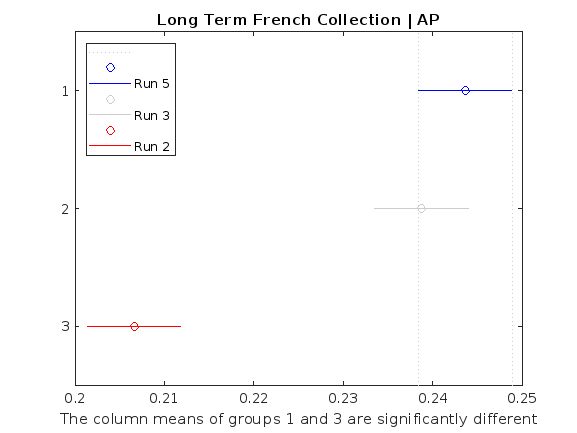
\includegraphics[width=\textwidth]{figure/StatisticalAnalysis/ANOVA 2/ap-lt-fr.jpeg}
      %\caption{\ac{AP} Two-way \ac{ANOVA} for Runs 2, 3, and 5 on the Long Term French Collection}
      \label{fig:lt_anova_french_ap}
    \end{subfigure}
    \caption{Two-way \ac{ANOVA} plots for the Runs on the French Collection}
    \label{fig:lt_anova_french}
  \end{figure}

Analyzing the two-way \ac{ANOVA} plot above, at first view we can notice, as expected, that there is no interaction among the three runs.  

Then, we observe that Run 5 consistently achieves the highest mean \ac{nDCG}  and \ac{AP} scores across different evaluation points. 
Run 2 exhibits lower performance compared to the other runs, while Run 3 shows a relatively stable performance, albeit slightly lower than Run 5, confirming what we found in Section \ref{sec:ndcg_comparison_french}.
In addition, the overlap we find among the columns of Run 3 and Run 5 suggests that the small changes done from Run 3 to Run 5 (see Table \ref{tab:run_parameters}) led to some noticeable albeit small improvements. 
These findings suggest that both the choice of run and the long-term evaluation have a significant impact on the overall \ac{nDCG} and \ac{AP} scores obtained.

To complement the two-way \ac{ANOVA} plot, we refer to Tables \ref{table:lt_anova_french} and \ref{table:lt_anova_french_ap}, that present additional statistical information.
providing multiple comparisons between the mean \ac{nDCG} and \ac{AP}, scores, variance, and p-values associated with runs 2, 3, and 5. 
The p-values indicate the level of significance and suggest whether there is a significant difference in performance between runs. 

The tables present the results of the pairwise comparisons between different runs. 
The "Group A" and "Group B" columns indicate the runs being compared. 
The "Lower Limit" and "Upper Limit" columns represent the lower and upper bounds of the confidence interval, while the "A-B" column indicates the mean difference between the runs. 
The "P-value" column displays the statistical significance of the comparison.

\newpage
\begin{table}[!h]
    \centering
    \caption{\ac{nDCG} Multiple Comparisons for Runs 2, 3, and 5 on the Long Term French Collection}
    \label{table:lt_anova_french}
    \begin{tabular}{cccccc}
    \hline
    Group A & Group B & Lower Limit & A-B & Upper Limit & P-value \\ \hline
    5 & 3 & -0.0023 & 0.0077 & 0.0177 & 0.1661 \\
    5 & 2 & 0.0305 & 0.0405 & 0.0505 & 1.16E-21 \\
    3 & 2 & 0.0228 & 0.0328 & 0.0428 & 3.84E-14 \\ \hline
    \end{tabular}
\end{table}

\begin{table}[!h]
    \centering
    \caption{\ac{AP} Multiple Comparisons for Runs 2, 3, and 5 on the Long Term French Collection}
    \label{table:lt_anova_french_ap}
    \begin{tabular}{cccccc}
    \hline
    Group A & Group B & Lower Limit & A-B & Upper Limit & P-value \\ \hline
    5 & 3 & -0.0057 & 0.0049 & 0.0154 & 0.523 \\
    5 & 2 & 0.0265 & 0.037 & 0.0476 & 0 \\
    3 & 2 & 0.0216 & 0.0322 & 0.0427 & 0 \\ \hline
    \end{tabular}
\end{table}

Looking at Table \ref{table:lt_anova_french}, the comparison between Run 5 and Run 3 yields a p-value of 0.1661, indicating that the mean difference in \ac{nDCG} scores between these runs is not statistically significant. 
Similarly, the comparison between Run 5 and Run 2 results in an extremely low p-value of 1.16E-21, suggesting a highly significant difference in \ac{nDCG} scores. 
Finally, the comparison between Run 3 and Run 2 also demonstrates a remarkably low p-value of 3.84E-14, indicating a significant discrepancy in their \ac{nDCG} scores.

These statistical results from the multiple comparisons provide further evidence of the differences in the retrieval performance among the runs on the Long Term French Collection. 
The significance of the mean differences confirms that the choice of run significantly affects the \ac{nDCG} scores. 
Additionally, the p-values obtained from the comparisons reinforce the observations made from the two-way \ac{ANOVA} plot, highlighting the superior performance of Run 5 and the relatively stable performance of Run 3 compared to the other runs.

\newpage
\enlargethispage{10\baselineskip}
\subsubsection{Two-way ANOVA on the Short Term French Collection}

Similarly, the results of the two-way \ac{ANOVA} for mean \ac{nDCG} and \ac{AP} performed on the Short Term French Collection are visualized in Figure \ref{fig:st_anova_french}. 

\begin{figure}[!h]
    \centering
    \begin{subfigure}[b]{0.49\textwidth}
        \centering
        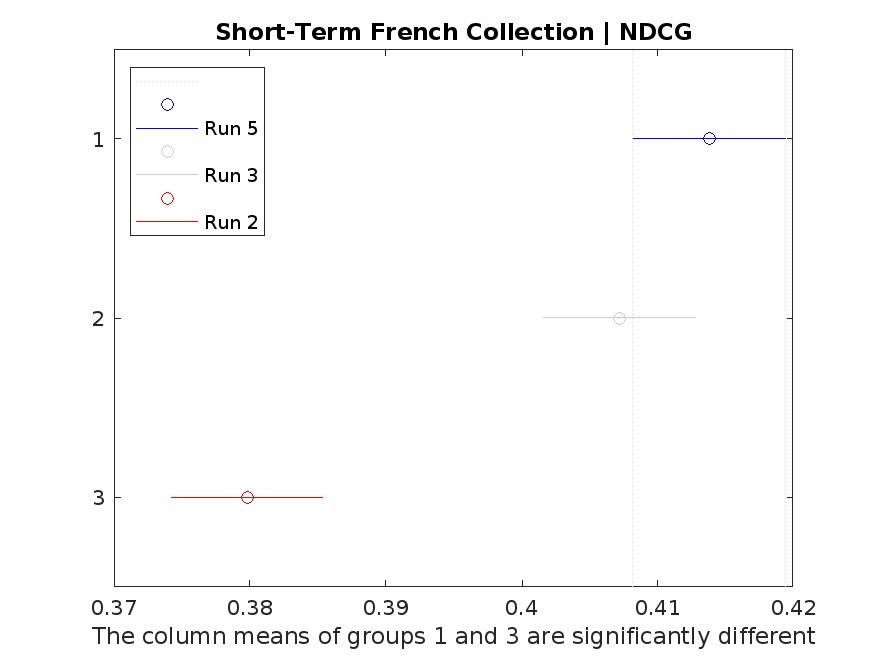
\includegraphics[width=\textwidth]{figure/StatisticalAnalysis/ANOVA 2/ndcg-st-fr.jpeg}
        %\caption{Two-way \ac{ANOVA} for Runs 2, 3, and 5 on the Short Term French Collection}
        \label{fig:st_anova_french_ndcg}        
    \end{subfigure}
    \hfill
    \begin{subfigure}[b]{0.49\textwidth}
        \centering
        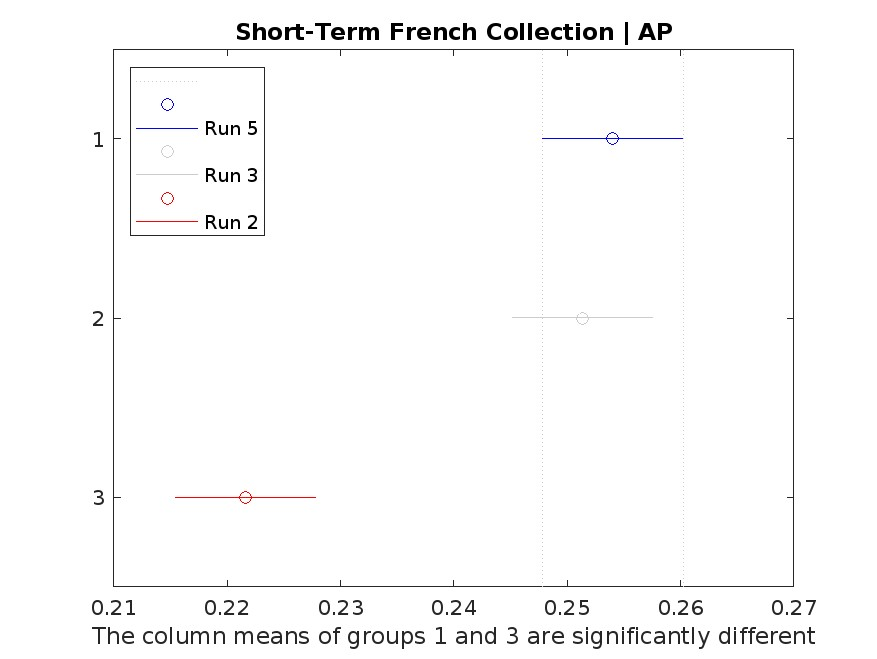
\includegraphics[width=\textwidth]{figure/StatisticalAnalysis/ANOVA 2/ap-st-fr.jpeg}
        %\caption{Two-way \ac{ANOVA} for Runs 2, 3, and 5 on the Short Term French Collection}
        \label{fig:st_anova_french_ap}
    \end{subfigure}
    \caption{Two-way \ac{ANOVA} for Runs 2, 3, and 5 on the Short Term French Collection}
    \label{fig:st_anova_french}
\end{figure}

The considerations made in Section \ref{sec:anova_fr_lt} hold in almost the same way for the results the system got on short-term Collection.  

To further investigate the statistical differences among the runs, we refer to the multiple comparisons Tables \ref{table:st_anova_french} and \ref{table:st_anova_french_ap} shown below, which uses the same notation as Table \ref{table:lt_anova_french}:

\begin{table}[!h]
    \centering
    \caption{\ac{nDCG} Multiple Comparisons for Runs 2, 3, and 5 on the Short Term French Collection}
    \label{table:st_anova_french}
    \begin{tabular}{cccccc}
    \hline
    Group A & Group B & Lower Limit & A-B & Upper Limit & P-value \\ \hline
    5 & 3 & -0.0047 & 0.0066 & 0.0178 & 0.355 \\
    5 & 2 & 0.0227 & 0.034 & 0.0452 & 3.86E-12 \\
    3 & 2 & 0.0162 & 0.0274 & 0.0386 & 3.33E-08 \\ \hline
    \end{tabular}
\end{table}

\begin{table}[!h]
    \centering
    \caption{\ac{AP} Multiple Comparisons for Runs 2, 3, and 5 on the Long Term French Collection}
    \label{table:st_anova_french_ap}
    \begin{tabular}{cccccc}
    \hline
    Group A & Group B & Lower Limit & A-B & Upper Limit & P-value \\ \hline
    5 & 3 & -0.0098 & 0.0027 & 0.0151 & 0.8701 \\
    5 & 2 & 0.0199 & 0.0324 & 0.0448 & $3.15 \times 10^{-9}$ \\
    3 & 2 & 0.0173 & 0.0297 & 0.0422 & $6.48 \times 10^{-8}$ \\ \hline
    \end{tabular}
\end{table}
 
Looking at Table \ref{table:st_anova_french}, the comparison between Run 5 and Run 3 yields a p-value of 0.355, indicating that the mean difference in \ac{nDCG} scores between these runs is not statistically significant. 
Similarly, the comparison between Run 5 and Run 2 results in a remarkably low p-value of 3.86E-12, suggesting a highly significant difference in \ac{nDCG} scores. 
Finally, the comparison between Run 3 and Run 2 also demonstrates a low p-value of 3.33E-08, indicating a significant discrepancy in their \ac{nDCG} scores.

In summary, the statistical analysis of the results obtained on the French collection reveals valuable insights into the performance of different runs. 
Run 5 has been multiple times confirmed to be the most effective one among the three, showing a noticeable overall strength in retrieving and ranking relevant documents.
This was easily predictable since this is the last and most elaborate and promising implementation we did for the French Collection, as discussed in Section \ref{sec:results}.   


\newpage
\enlargethispage{8\baselineskip}
\subsection{Analysis of Results on the English Collection}

\subsubsection{Overall \textit{nDCG} Comparison} \label{sec:ndcg_comparison_eng}

The overall \ac{nDCG} comparison for Runs 1 and 4 on the English collection is depicted in Figure \ref{fig:overall_ndcg_eng}, which uses the same notation as Figure \ref{fig:overall_ndcg_french_boxplot}.

\begin{figure}[!h]
\centering
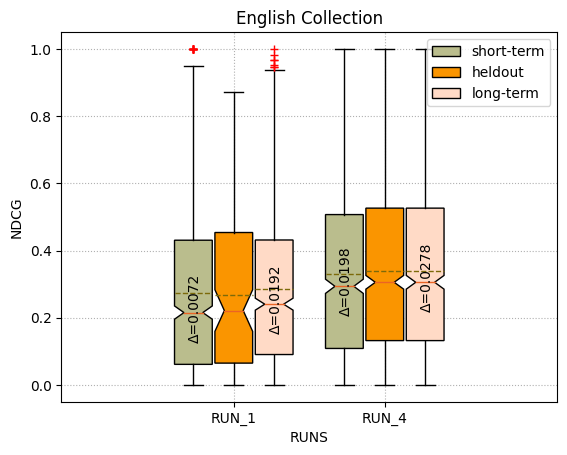
\includegraphics[width=0.8\textwidth]{figure/StatisticalAnalysis/BoxPlot/NDGC ENGLISH.png}
\caption{Overall nDCG Comparison for Runs 1 and 4 on the English Collection}
\label{fig:overall_ndcg_eng}
\end{figure}
 
Upon analyzing the overall \ac{nDCG} comparison, we first notice that the results on the English Collection are notably worse compared to those observed for the French Collection in Section \ref{sec:ndcg_comparison_french}. 
This discrepancy is not unexpected, since the focus of our work was primarily on improving the retrieval performance of our \ac{IR} system on the French Collection.

Examining the boxplot in Figure \ref{fig:overall_ndcg_eng}, we can observe that Run 4 consistently outperforms Run 1 and achieves higher \ac{nDCG} scores across both the Short and Long Term evaluations on the English Collection.  
The clear separation between the two runs in the boxplot suggests significant differences in their retrieval performance, indicating the superior effectiveness of Run 4 in retrieving relevant documents.

Furthermore, by considering the \ac{RnD} deltas represented by the values inside the boxes, we can observe that Run 4 exhibits a good level of stability between the Short and Long Term evaluations, with minimal changes in its \ac{nDCG} scores. 
On the other hand, Run 1 shows a notable increase in \ac{RnD} from the Short to the Long Term, more than doubling the delta value. 
This indicates that Run 1's performance significantly deteriorates when transitioning from the Short to the Long Term evaluation of the English Collection.

In summary, the overall \ac{nDCG} comparison confirms that Run 4 performs better than Run 1 in all evaluation settings on the English Collection. 
Run 4 demonstrates higher \ac{nDCG} scores and exhibits greater stability between the Short and Long Term evaluations, while Run 1 experiences a noticeable decline in performance when moving from the Short to the Long Term. 
These findings highlight the importance of the improvements achieved in Run 4 and emphasize its superior retrieval effectiveness compared to Run 1.

\newpage
\enlargethispage{6\baselineskip}
\subsubsection{Overall \textit{MAP} Comparison} \label{sec:map_comparison_eng}

We now turn our attention to the overall \ac{MAP} comparison of Runs 1 and 4 on the English collection, as illustrated in Figure \ref{fig:map_english}. 
The boxplot showcases the distribution of \ac{MAP} scores, using the same notation as Figure \ref{fig:map_french}.

\begin{figure}[!h]
\centering
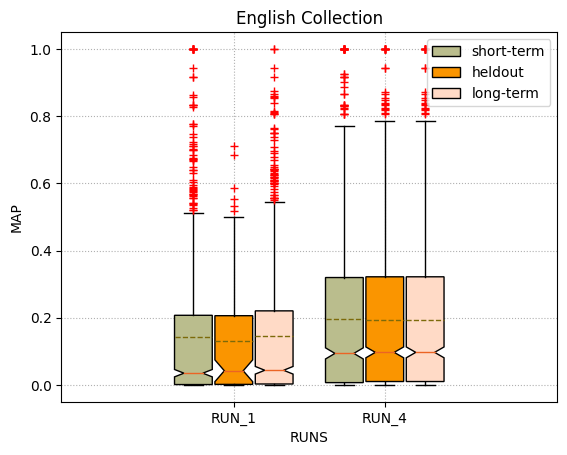
\includegraphics[width=0.8\textwidth]{figure/StatisticalAnalysis/BoxPlot/MAP English.png}
\caption{Overall \ac{MAP} Comparison of Runs 1 and 4 on the English Collection}
\label{fig:map_english}
\end{figure}
 
Analyzing the boxplot in Figure \ref{fig:map_english}, we observe that Run 4 consistently outperforms Run 1 on all three collections: Short Term, Heldout, and Long Term. 
Run 4 exhibits higher median \ac{MAP} scores in both the Short Term and Long Term evaluations, indicating its superior retrieval performance in terms of average precision across different evaluation points.

Although the distribution of \ac{MAP} scores for Run 1 appears to be more concentrated, suggesting more consistent performance, Run 4 clearly demonstrates better overall effectiveness in retrieving relevant documents on the English Collection.

However, in terms of the Heldout Collection, both Runs 1 and 4 display comparable median \ac{MAP} scores, indicating similar retrieval performance within this collection. 

These findings reinforce the conclusions drawn in Section \ref{sec:ndcg_comparison_eng} regarding the superior performance of Run 4 compared to Run 1 on the English Collection. 


\newpage
\enlargethispage{8\baselineskip}
\subsubsection{Two-way \textit{ANOVA} on the Long Term English Collection}

The results of the two-way \ac{ANOVA} performed on the Long Term English Collection are shown in Figure \ref{fig:lt_anova_eng}, which illustrates the mean \ac{nDCG} and \ac{AP} scores for Run 1 in red on the left and Run 4 in blue on the right. 

\begin{figure}[!h]
    \centering
    \begin{subfigure}[b]{0.49\textwidth}
        \centering
        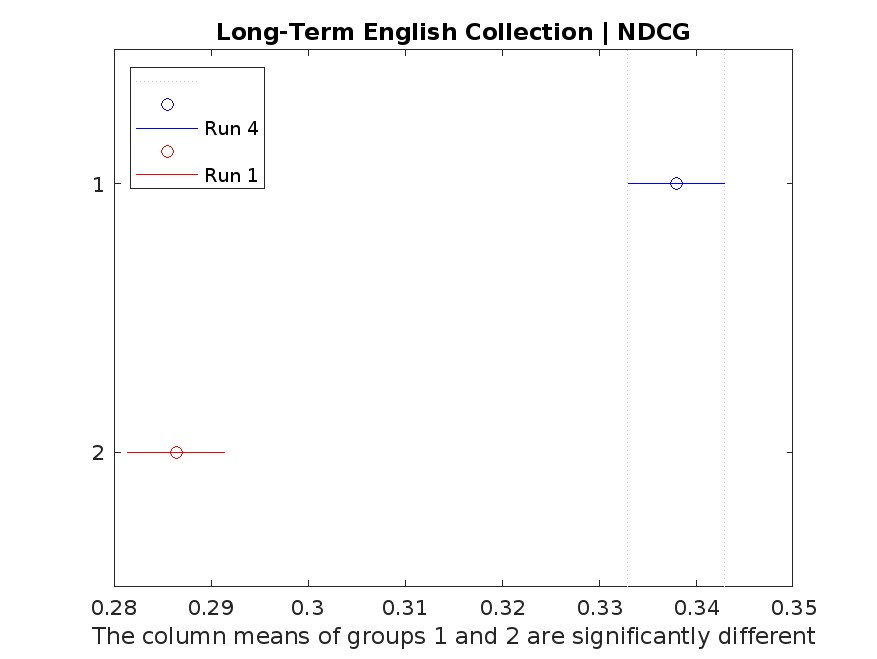
\includegraphics[width=\textwidth]{figure/StatisticalAnalysis/ANOVA 2/ndcg-lt-en.jpeg}
        %\caption{Two-way ANOVA for Runs 1 and 4 on the Long Term English Collection}
        \label{fig:lt_anova_eng_ndcg}
    \end{subfigure}
    \hfill
    \begin{subfigure}[b]{0.49\textwidth}
        \centering
        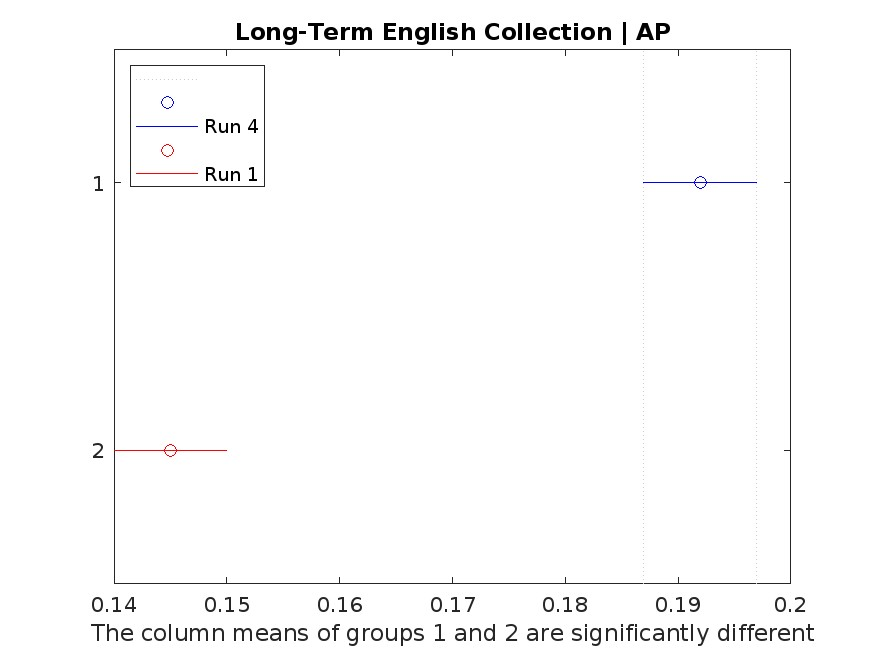
\includegraphics[width=\textwidth]{figure/StatisticalAnalysis/ANOVA 2/ap-lt-en.jpeg}
        %\caption{Two-way ANOVA for Runs 1 and 4 on the Long Term English Collection}
        \label{fig:lt_anova_eng_ap}
    \end{subfigure}
    \caption{Two-way ANOVA for Runs 1 and 4 on the Long Term English Collection}
    \label{fig:lt_anova_eng}
\end{figure}

At first, we can see that, as expected, there is no interaction between these two runs. To reinforce this, we can also see that there is no overlap between their column means.

Continuing into analyzing the two-way \ac{ANOVA} plot, we find that Run 4 achieves higher mean \ac{nDCG} scores compared to Run 1 across different evaluation points. 
This suggests the superiority of Run 4 in retrieving relevant documents in the long term on the English collection, keep confirming what we found in Section \ref{sec:ndcg_comparison_eng}. 

To provide additional statistical information, we refer to Tables \ref{table:lt_anova_eng} and \ref{table:lt_anova_eng_ap}, which present the results of multiple comparisons between Run 1 and Run 4 for the Long Term English Collection. 
The table shows the lower limit, A-B difference, upper limit, and p-value for the comparison. 
In this case, there is a single row in the table since there is only one comparison between the two runs.

\begin{table}[!h]
    \centering
    \caption{\ac{nDCG} Multiple comparisons for the Long Term English Collection}
    \label{table:lt_anova_eng}
    \begin{tabular}{cccccc}
    \hline
    Group A & Group B & Lower Limit & A-B Difference & Upper Limit & P-value \\
    \hline
    4 & 1 & 0.0415 & 0.0515 & 0.0615 & $6.77 \times 10^{-25}$ \\
    \hline
    \end{tabular}
\end{table}

\begin{table}[!h]
    \centering
    \caption{\ac{AP} Multiple comparisons for the Long Term English Collection}
    \label{table:lt_anova_eng_ap}
    \begin{tabular}{cccccc}
    \hline
    Group A & Group B & Lower Limit & A-B Difference & Upper Limit & P-value \\
    \hline
    4 & 1 & 0.0369 & 0.0469 & 0.057 & $2.13 \times 10^{-20}$ \\
    \hline
    \end{tabular}
\end{table}
    
Table \ref{table:lt_anova_eng} suggests a significant difference between Run 1 and Run 4 in terms of \ac{nDCG} scores for the Long Term English Collection. 
The positive A-B difference and the large p-value indicate that Run 4 consistently achieves higher \ac{nDCG} scores than Run 1 across different evaluation points.

These findings further support the conclusion that Run 4 performs better than Run 1 in terms of retrieving relevant documents over the long term on the English collection, as discussed in Sections \ref{sec:ndcg_comparison_eng} and \ref{sec:map_comparison_eng}.


\newpage
\enlargethispage{5\baselineskip}
\subsubsection{Two-way \textit{ANOVA} on the Short Term English Collection}

Similarly, the results of the two-way \ac{ANOVA} for mean \ac{nDCG} and \ac{AP} performed on the Short Term English Collection are depicted in Figure \ref{fig:st_anova_eng}.

\begin{figure}[!h]
    \centering
    \begin{subfigure}[b]{0.49\textwidth}
        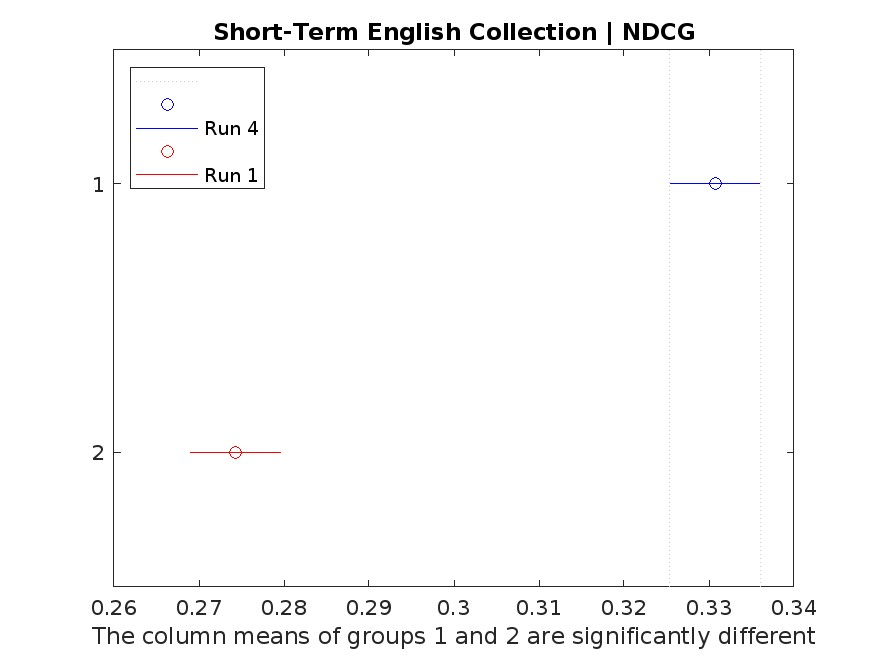
\includegraphics[width=\textwidth]{figure/StatisticalAnalysis/ANOVA 2/ndcg-st-en.jpeg}
        %\caption{Two-way ANOVA for Runs 2 and 4 on the Short Term English Collection}
        \label{fig:st_anova_eng_ndcg}        
    \end{subfigure}
    \hfill
    \begin{subfigure}[b]{0.49\textwidth}
        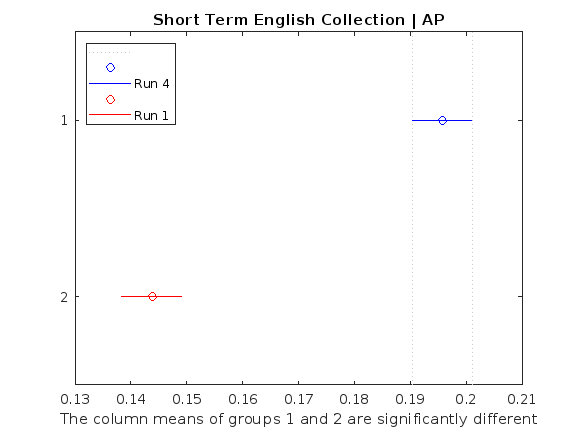
\includegraphics[width=\textwidth]{figure/StatisticalAnalysis/ANOVA 2/ap-st-en.jpeg}
        %\caption{Two-way ANOVA for Runs 2 and 4 on the Short Term English Collection}
        \label{fig:st_anova_eng_ap}
    \end{subfigure}
    \caption{Two-way ANOVA for Runs 1 and 4 on the Short Term English Collection}
    \label{fig:st_anova_eng}
\end{figure}
 
These results confirm everything we have found until now, indicating the superiority of run 4 on both Short Term and Long Term Collection.

To provide additional statistical information, Tables \ref{table:st_anova_eng} and \ref{table:st_anova_eng_ap} present the results of the multiple comparisons between Run 1 and Run 4.

\begin{table}[!h]
    \centering
    \caption{Multiple comparisons for the Short Term English Collection}
    \label{table:st_anova_eng}
    \begin{tabular}{cccccc}
    \hline
    Group A & Group B & Lower Limit & A-B Difference & Upper Limit & P-value \\
    \hline
    4 & 1 & 0.0457 & 0.0564 & 0.0671 & $0.00 \times 10^{0}$ \\
    \hline
    \end{tabular}
\end{table}

\begin{table}[!h]
    \centering
    \caption{Multiple comparisons for the Short Term English Collection}
    \label{table:st_anova_eng_ap}
    \begin{tabular}{cccccc}
    \hline
    Group A & Group B & Lower Limit & A-B Difference & Upper Limit & P-value \\
    \hline
    4 & 1 & 0.0412 & 0.052 & 0.0628 & $1.05 \times 10^{-21}$ \\
    \hline
    \end{tabular}
\end{table}

Table \ref{table:st_anova_eng} shows that there is a significant difference in the mean \ac{nDCG} scores between Run 1 and Run 4 on the Short Term English Collection. 
The A-B difference, which represents the difference in \ac{nDCG} scores between the two runs, is 0.0564, indicating that Run 4 performs substantially better than Run 1. 
The p-value, which is practically zero, further supports the significance of this difference.

These findings consistently demonstrate the superiority of Run 4 over Run 1 in terms of \ac{nDCG} scores in both short and long-term evaluations of the English collection.


\newpage
\enlargethispage{4\baselineskip}
\subsection{Final Considerations on Statistical Analysis}

In this section, we conducted a comprehensive statistical analysis of the retrieval performance of our system on both the French and English collections. 
We focused on evaluating the overall \ac{nDCG} and \ac{MAP} scores, as well as conducting two-way \ac{ANOVA} tests to examine the effects of different factors on the performance.

For the French collection, we compared the performances of Runs 2, 3, and 5. 
The analysis revealed that Run 5 consistently exhibited slightly better or comparable performance compared to Run 3 across all evaluation points. 
This suggests that the modifications made in Run 5 resulted in improved retrieval effectiveness, making it a promising option. 
On the other hand, Run 2 displayed significantly worse performance compared to the other runs, indicating the need for further improvements.

Turning to the English collection, we focused on comparing Runs 1 and 4. 
The results consistently demonstrated that Run 4 outperformed Run 1 in every aspect of the analysis. 
It achieved higher \ac{nDCG} scores, indicating its superior effectiveness in retrieving relevant documents. 
Additionally, Run 4 displayed a higher median \ac{MAP} score, indicating its superior overall performance in both short and long windows of time. 
These findings establish Run 4 as the more successful option for retrieval on the English collection.

The two-way \ac{ANOVA} tests further supported our conclusions. 
In the French collection, the two-way \ac{ANOVA} analysis confirmed the superiority of Run 5 over Run 3 in terms of \ac{nDCG} scores. 
This finding aligns with the overall comparison results. 

In the English collection, the two-way \ac{ANOVA} did not provide any new unexpected result, as the performance differences between Run 1 and Run 4 were consistently evident in all previous aspects of the analysis.

In summary, our statistical analysis highlights the varying performances of different runs in the French and English collections. 
For the French collection, Run 5 exhibited slightly better or comparable performance compared to Run 3, while Run 2 displayed significantly worse performance. 
In contrast, for the English collection, Run 4 consistently outperformed Run 1 in every aspect of the analysis.

































